\documentclass[11pt]{extarticle}

\usepackage[english,french]{babel}
\usepackage[utf8]{inputenc}
\usepackage{url}
\usepackage[T1]{fontenc}
\usepackage{booktabs}
\usepackage{enumitem}
\usepackage{graphicx}
\usepackage{pifont}
\usepackage{makecell}
\setcellgapes{1pt}
\usepackage{placeins}
\usepackage{subcaption}
\usepackage{pgfplots}
\usetikzlibrary{calc}
\pgfplotsset{compat=1.18}
\usepgfplotslibrary{dateplot}
\usepackage[margin=1in]{geometry}
\usepackage[colorlinks=true, allcolors=blue]{hyperref}
\usepackage{amsmath}
\usepackage{pgfplotstable}
\usepackage{amsfonts}
\usepgfplotslibrary{groupplots}

\usetikzlibrary{backgrounds}

% Configuration de pgfplotstable
\pgfplotstableset{
    col sep=comma, % Colonnes séparées par des virgules
    string type,
    every head row/.style={
        before row=\toprule,
        after row=\midrule},
    every last row/.style={after row=\bottomrule},
}

\title{
    \hspace*{-12cm}
    \vspace*{1cm}
    \protect\\
    \vspace*{1cm}
    \textbf{Long Term Memory Processes Using Hurst Estimation}
}

\author{Remiat Alexandre}

\date{\today}

\graphicspath{{img/}}

\xdefinecolor{kblue}{RGB}{0,38,69}
\xdefinecolor{korange}{RGB}{255,128,89}
\xdefinecolor{kgray}{RGB}{47,108,130}
\xdefinecolor{kgreen}{RGB}{102,143,72}


\begin{document}

\selectlanguage{english}

\maketitle


\newpage


\section*{Abstract}

This paper presents a study on long-term memory processes in financial time series using Hurst estimation methods,
specifically the traditional R/S statistic (Rescaled Range analysis) and the modified R/S statistic.
The R/S statistic and the modified R/S statistic are computed to determine the presence of long-range dependence in the time series data.
Unfortunately, the results are not very conclusive, as the single Hurst exponent computed for the whole series is not a very robust statistic and can be
influenced by the length of the series, the presence of trends, or structural breaks.
To address these issues, we employed the Multifractal Detrended Fluctuation Analysis (MF-DFA) to investigate the
local behavior of the series and characterize its singularity spectrum. The multifractal spectrum reveals that the series
might exhibits multifractal properties. To take advantage of this, we propose a trading strategy based on the Hurst
exponent and the singularity spectrum, where we look into pairs with different scaling behavior (S\&P 500 and Russell 2000).
The results are encouraging, as the strategy outperforms the long-only S\&P 500 portfolio and the long-only Russell 2000 portfolio.
Again, those results are to take with a grain of salt, as multifractal analysis requires a lot of data points to be
reliable and this analysis should be extended to other pairs of assets to confirm the results.


\newpage

\section{Introduction}

The Hurst exponent is a crucial tool for analyzing long-term memory and self-similarity in stochastic processes. Originally introduced by Harold Hurst in the 1950s for studying river flows, this measure has since been widely adopted in various fields such as finance, physics, and environmental science. In financial markets, the Hurst exponent serves as an indicator to determine whether a time series exhibits long-range dependence (a value greater than 0.5) or mean-reverting behavior (a value less than 0.5).

The most common method for estimating the Hurst exponent is through Rescaled Range (R/S) analysis, introduced by Hurst and later refined by Mandelbrot. However, the traditional R/S statistic has its limitations, particularly its sensitivity to short-term memory effects, which can obscure the detection of long-term dependencies. To mitigate these issues, Lo (1991) proposed a modified version of the R/S statistic (M-R/S) that better accounts for short-term autocorrelation.

In this study, we apply both the R/S method and the M-R/S to estimate the Hurst exponent on financial time series and we complement our analysis with Multifractal Detrended Fluctuation Analysis (MF-DFA), which examines the local behavior of the series and characterizes its singularity spectrum.

The Fractional Brownian motion (fBm) is often used as a benchmark model for processes with memory, as it embodies the scaling properties and persistence typically observed in long-memory data. While fBm provides a theoretical framework for understanding these phenomena, our study focuses on practical estimation methods.

\section{Fractional Brownian Motion}

Fractional Brownian motion (fBm) is a generalization of standard Brownian motion that introduces dependence in increments,
making it suitable for modeling processes with memory effects. It is a continuous-time Gaussian process \( X_H(t) \) H corresponds
to the Hurst exponent and \( H \in [0, 1] \) with the following properties:

\begin{itemize}
    \item \( X_H(0) = 0 \).
    \item The increments \( X_H(t) - X_H(s) \) follow a normal distribution with mean zero and variance \sigma^2:
    \begin{equation}
        \mathbb{E} \left[ (X_H(t) - X_H(s))^2 \right] = \sigma^2|t - s|^{2H},
    \end{equation}
    where \( H \) is the Hurst exponent.
    \item The process exhibits self-similarity, meaning that for any scaling factor \( c \), \( c \in \mathbb{R}^+ \), the rescaled process satisfies:
    \begin{equation}
        X_H(ct) \overset{d}{=} c^H X_H(t).
    \end{equation}
    where the symbol \(\stackrel{d}{=}\) denotes equality in distribution, meaning that the statistical properties of \(X_H(ct)\) and \(c^H X_H(t)\) are identical.

    \item When \( H = 0.5 \), fBm reduces to classical Brownian motion.
    \item For \( H > 0.5 \), the process exhibits long-term positive autocorrelation, meaning that an increase in the past tends to be followed by further increases.
    \item For \( H < 0.5 \), the process has anti-persistent behavior, where an increase in the past is more likely to be followed by a decrease.
\end{itemize}

The covariance function of fBm is given by:

\begin{equation}
    C_H(t_1, t_2) = \frac{\sigma^2}{2} \left( t_1^{2H} + t_2^{2H} - |t_1 - t_2|^{2H} \right),
    \label{eq:fbm_covariance}
\end{equation}

which accounts for the dependence structure of the process. The Hurst exponent \( H \) plays a critical role in determining the smoothness and correlation properties of fBm:

\begin{itemize}
    \item \textbf{For small \( H \) values} (\( H < 0.5 \)), the process is highly erratic, with rapid changes and weak memory effects.
    \item \textbf{For large \( H \) values} (\( H > 0.5 \)), the trajectory becomes smoother, and the process exhibits long-range dependence.
\end{itemize}

Fractional Brownian motion is widely used in finance, telecommunications, and physics to model phenomena exhibiting memory effects and self-similarity, such as stock market fluctuations, internet traffic, and geological formations.


\subsection{Simulation of Fractional Brownian Motion}

To generate the fractional Brownian motion (fBm), we use a Cholesky decomposition-based approach. The covariance matrix of fBm is given by \eqref{eq:fbm_covariance}:

where \( H \) is the Hurst exponent, which determines the degree of long-term dependence in the process.

The steps of the simulation are as follows:
\begin{enumerate}
    \item Define a time grid of \( N \) points between \( 0 \) and \( T \).
    \item Compute the covariance matrix using the formula above.
    \item Apply Cholesky decomposition to obtain a lower triangular matrix \( L \).
    \item Generate a vector \( W \) of standard normal random variables.
    \item Obtain the fBm path by computing \( X = L W \).
\end{enumerate}

The params used for this simulation are N = 1000, T = 1, and Hurst exponents \( H = 0.2, 0.3, 0.5, 0.6, 0.8 \), the number
of lag for the autocorrelation is 40.

\begin{figure}[!ht]
    \centering
    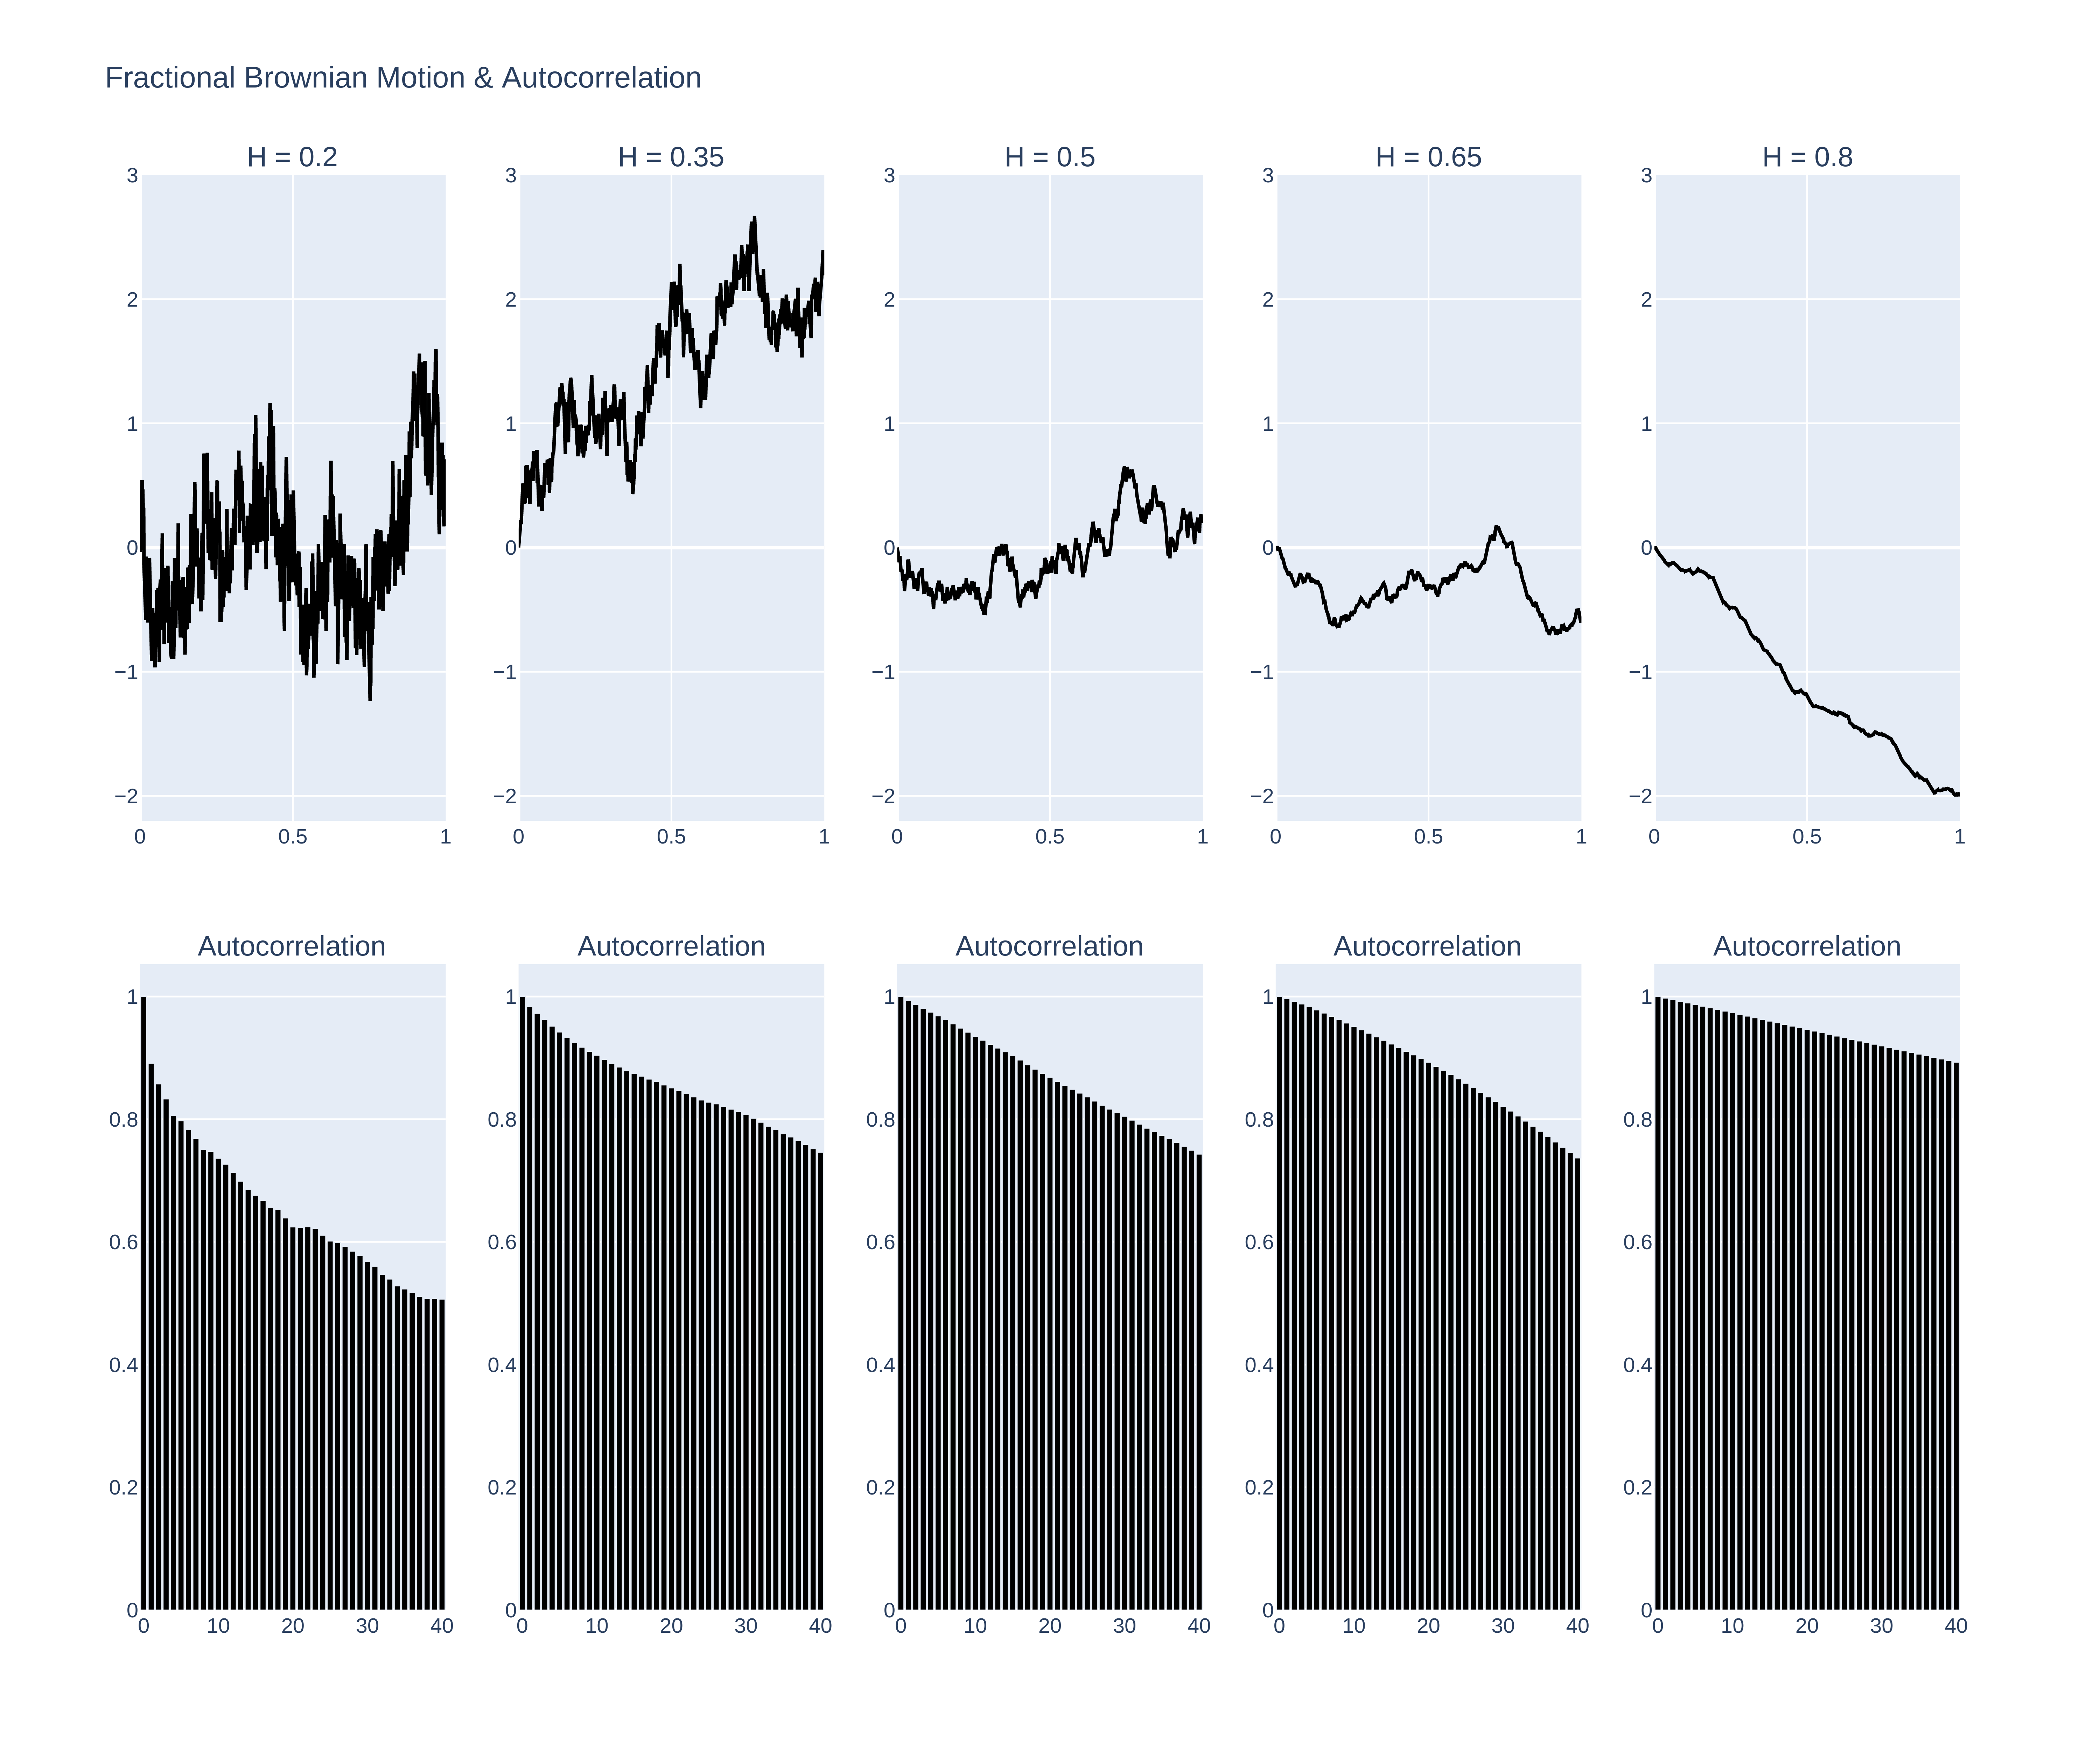
\includegraphics[width=0.8\textwidth]{img/fdm_autocorr}
    \caption{Simulation of Fractional Brownian Motion with different Hurst exponent and its autocorrelation function.}
    \label{fig:fbm_autocorr}
\end{figure}

\FloatBarrier

The behavior of the fractional Brownian motion (fBm) varies significantly with the Hurst exponent \( H \).

When \( H \) is small (close to 0), the fBm exhibits high local variability, resulting in a highly granular trajectory with frequent fluctuations. The autocorrelation of increments decays rapidly, indicating that future values are weakly influenced by past values. This suggests a short-memory process, similar to standard Brownian motion.

As \( H \) increases, the autocorrelation decays more slowly, meaning that past values have a more significant impact on future values. This introduces a form of long-term dependence, where the process exhibits persistent trends. Consequently, the fBm trajectory appears smoother, with larger coherent movements and fewer abrupt changes.

In summary, a lower \( H \) leads to a more irregular and noisy path, characteristic of short-memory processes, while a higher \( H \) results in a smoother trajectory with stronger persistence.

\subsection{Hurst exponent Calculation}
\subsection{R/S and modified R/S Analysis}
The R/S (Rescaled Range) analysis, introduced by Hurst and developed in various works by Mandelbrot, is certainly the most well-known method for estimating the Hurst exponent $H$. This statistic is defined as the range of the partial sums of deviations from the mean of a time series divided by its standard deviation. Consider a time series $Y_t$, $t = 1, ..., T$, with mean $\bar{Y}$. The range $R$ is defined as:

\[
R = \max_{1 \leq j \leq T} \left( Y_j - \bar{Y} \right) - \min_{1 \leq j \leq T} \left( Y_j - \bar{Y} \right)
\]

The R/S statistic is then computed by dividing the range by the standard deviation $s_T$ of the series:

\[
Q_T = \frac{R}{s_T} = \frac{\max_{1 \leq j \leq T} \left( Y_j - \bar{Y} \right) - \min_{1 \leq j \leq T} \left( Y_j - \bar{Y} \right)}{s_T}, \quad \text{with } s_T = \sqrt{\frac{1}{T} \sum_{j=1}^{T} \left( Y_j - \bar{Y} \right)^2}.
\]


Empirical studies by Mandelbrot and Wallis (1969e) have shown that \( Q_T \) scales with the number of observations \( T \) according to
\[
Q_T \sim T^H,
\]
which implies that by taking logarithms, the Hurst exponent \( H \) can be obtained from
\[
H = \frac{\log(Q_T)}{\log(T)}.
\]


\subsection{Modified R/S Analysis}
The modified R/S statistic, denoted by $\tilde{Q}_T$, is defined as:

\[
\tilde{Q}_T = \frac{R}{\hat{\sigma}_T(q)}
\]

where

\[
\hat{\sigma}_T(q) = \sqrt{\frac{1}{T} \sum_{j=1}^{T} (Y_j - \bar{Y})^2 + \frac{2}{T} \sum_{j=1}^{T} w_j(q) \left[ \sum_{i=j+1}^{T} (Y_i - \bar{Y})(Y_{i-j} - \bar{Y}) \right]}
\]

and

\[
w_j(q) = 1 - \frac{j}{q + 1}
\]

This statistic differs from the traditional R/S statistic only by its denominator. In the presence of autocorrelation,
the denominator does not only represent the sum of the variances of the individual terms, but also includes autocovariances.
These are weighted according to lags $q$, with the weights $w(q)$ suggested by Newey and West (1987). Moreover, Andrews
(1991) proposed a rule for choosing $q$:

\[
q = \left[ k_T \right] \quad \text{where} \quad k_T = \left( \frac{3T}{2} \right)^{1/3} \left( \frac{2 \rho_1}{1 - \rho_1^2} \right)^{2/3}
\]

where $[k_T]$ is the integer part of $k_T$, and $\rho_1$ is the first-order autocorrelation coefficient.

Unlike the classical R/S analysis, the limiting distribution of the modified R/S statistic is known, and the statistic $V$, defined by

\[
V = \frac{\tilde{Q}_T}{\sqrt{T}},
\]

converges to the range of a Brownian bridge over the unit interval. It is therefore possible to perform a statistical
test for the null hypothesis of short memory against the alternative hypothesis of long memory by referring to the
critical value table provided by Lo (1991), shown in Table~\ref{table:critical_values}.

\subsection{Data}

The data used in this analysis is montlhy and consists of the historical closing prices of five major stock market indices: the S\&P 500,
Russell 2000, FTSE 100, Nikkei 225, and the DAX.
The data spans the period from September 10th, 1987, to February 28, 2025, and was downloaded from Yahoo Finance.

For each index, the closing price time series was transformed using the natural logarithm to obtain a series of log returns.
Additionally, a stationarity test was conducted on the log return series using the Augmented Dickey-Fuller (ADF) test.
The results indicated that all series were non-stationary, suggesting the presence of unit roots. To address this, the series were differenced once, after which they exhibited stationarity.

These log returns were then used to calculate the R/S and modified R/S statistics and estimate the Hurst exponent.
The purpose of using this data is to evaluate the long-term memory properties of financial markets, which can indicate persistence or mean-reversion in market behavior.



\subsection{Results}

The following table summarizes the results of the R/S statistic, modified R/S statistic, and the estimated Hurst exponents for each of the five indices analyzed: \\

\begin{table}[h!]
    \centering
    \pgfplotstabletypeset[
        col sep=comma,
        header=true,
        string type,
        every head row/.style={before row=\hline, after row=\hline},
        every last row/.style={after row=\hline},
        columns/Ticker/.style={column name=Ticker, string type},
        columns/R/S Statistic/.style={column name=R/S Statistic, fixed, precision=2},
        columns/Hurst exponent (RS)/.style={column name=Hurst exponent (RS), fixed, precision=3},
        columns/modified Hurst exponent/.style={column name=modified Hurst exponent, fixed, precision=3},
        columns/critical value/.style={column name=critical value, fixed, precision=3},
        columns/long memory/.style={column name=long memory}
    ] {data/Hurst_results.csv}
    \caption{Results for R/S, Hurst exponent, modified Hurst exponent, critical value at 10\%, and rejection of the null
    hypothesis of long memory. The Hurst exponent can be equal for the R/S and modified R/S methods in the case where
    the autocorrelation coefficients are less than zero, in this case we set $q$ equal to 0 and therefore the R/S and modified R/S share the same formula.}
    \label{tab:Hurst_results}
\end{table}

\FloatBarrier


Based on the results obtained from applying the traditional R/S method, all the series appear to exhibit long-term memory,
as the Hurst exponents are consistently greater than 0.5. However, the asymptotic distribution of this statistic is unknown,
which prevents us from determining whether the estimated Hurst exponent is significantly greater than 0.5. This issue can be
addressed by using the modified R/S method. In this case, we simply compare the estimated values of the statistic V to the
critical values provided by Lo (1991), which are 1.620 and 1.747 for the 10\% and 5\% significance levels, respectively,
in the case of a one-tailed test. It is observed that only one serie actually exhibit persistence: the returns of the
Russell 2000 small and mid cap (US).
For all other series, despite the Hurst exponent being greater than 0.5, the null hypothesis
of short memory cannot be rejected.
From now on, we will focus on the Russell 2000 index because it seems like their is a long term memory caracteristics.


\subsection{Pitfalls and more granular analysis on the Russell 2000}

Unfortunately those results are not very conclusive, the static Hurst exponent is not a very robust statistic and can be
influenced by the length of the series, the presence of trends, or the presence of structural breaks.
To highlight these shortcomings, we adjust both the analysis frequency and the study period. Specifically, we perform a
detailed investigation across different frequencies (daily, weekly, monthly) and various study periods, comparing the
outcomes. This combined approach enables us to detect long-memory behavior within particular timeframes and ensures
more robust and reliable conclusions.

\begin{table}[h!]
    \centering
    \pgfplotstabletypeset[
        col sep=comma,
        header=true,
        string type,
        every head row/.style={before row=\hline, after row=\hline},
        every last row/.style={after row=\hline},
        columns/Frequency/.style={column name=Frequency, string type},
        columns/Hurst exponent/.style={column name=Hurst exponent, fixed, precision=2},
        columns/modified Hurst exponent/.style={column name=modified Hurst exponent, fixed, precision=3},
        columns/critical value/.style={column name=critical value, fixed, precision=3},
        columns/long memory/.style={column name=long memory, fixed, precision=3},
    ] {data/frequencies_results.csv}
    \caption{Results for Hurst exponent, modified Hurst exponent, critical value at 10\% and rejection of the null
    hypothesis of long memory, different frequencies daily, weekly and montlhy.}
    \label{tab:frequencies_results}
\end{table}

\FloatBarrier

\begin{table}[h!]
    \centering
    \pgfplotstabletypeset[
        col sep=comma,
        header=true,
        string type,
        every head row/.style={before row=\hline, after row=\hline},
        every last row/.style={after row=\hline},
        columns/Period/.style={column name=Period, string type},
        columns/Hurst exponent/.style={column name=Hurst exponent, fixed, precision=2},
        columns/modified Hurst exponent/.style={column name=modified Hurst exponent, fixed, precision=3},
        columns/critical value/.style={column name=critical value, fixed, precision=3},
        columns/long memory/.style={column name=long memory, fixed, precision=3},
    ] {data/timestamp_analysis.csv}
    \caption{Results for Hurst exponent, modified Hurst exponent, critical value at 10\% and rejection of the null
    hypothesis of long memory, different estimation periods.}
    \label{tab:timestamp_analysis}
\end{table}

\FloatBarrier

The results indicate that the detection of long memory strongly depends on the frequency and period of analysis.
At daily and weekly frequencies, the Hurst exponents are close to 0.5, suggesting no long memory, while at the monthly
frequency, a persistent behavior is detected (H = 0.645). Regarding estimation periods, only the longest period
(1987-2025) indicates long memory, whereas more recent periods reject this hypothesis. This suggests that long memory
may be an unstable characteristic influenced by structural trends or market changes.


The long memory properties of the Russell 2000 index are not stable over time and may be influenced by
structural changes or market dynamics. Given that the presence of long memory is not a consistent feature of the series,
it is necessary to delve into a more nuanced analysis.


Specifically, we will employ Multifractal Detrended Fluctuation Analysis (MF-DFA) to investigate the local behavior of
the series and to characterize its singularity spectrum. This method will allow us to uncover potential multifractal
properties and provide deeper insights into the complex, scale-dependent dynamics governing the index.




\section{Multifractal Detrended Fluctuation Analysis}

The Multifractal Detrended Fluctuation Analysis (MF-DFA) is a generalization of the standard DFA approach designed to detect multifractality in time series proposed by (Jan W. Kantelhardt (2002)). The procedure can be summarized in five steps, as described below:

\begin{enumerate}
    \item \textbf{Profile construction.} Given a series $\{x_k\}_{k=1}^N$, we define its mean  \(\bar{x}\). We build the profile
    \[
        Y(i) \;=\; \sum_{k=1}^{i} \bigl(x_k \;-\; \bar{x}\bigr),
        \quad i \;=\; 1,2,\dots,N.
    \]
    This cumulative sum helps to capture the local fluctuations in the data.

    \item \textbf{Division into segments.} We split the profile $Y(i)$ into $N_s \equiv \lfloor N/s \rfloor$ non-overlapping segments, each of length $s$. Since $N$ may not be a multiple of $s$, we repeat this procedure also starting from the opposite end, yielding $2\,N_s$ segments in total.

    \item \textbf{Detrending.} For each of the $2\,N_s$ segments, we fit a polynomial trend (often linear or quadratic) and subtract it from $Y(i)$ in that segment. Let $y_\nu(i)$ be the fitting polynomial in segment $\nu$. We then define the local variance
    \[
        F^2\bigl(s,\nu\bigr)
        \;=\;
        \frac{1}{s}
        \sum_{i=1}^s
        \Bigl[\,Y\bigl((\nu-1)s + i\bigr)\;-\;y_\nu(i)\Bigr]^2.
    \]
    This detrending removes possible polynomial trends in the data.

    \item \textbf{Generalized fluctuation function.} We compute, for each scale $s$, the $q$th-order fluctuation function,
    \[
        F_q(s)
        \;=\;
        \biggl\{
          \frac{1}{2\,N_s}
          \sum_{\nu=1}^{2\,N_s}
          \Bigl[
            F^2\bigl(s,\nu\bigr)
          \Bigr]^{\!q/2}
        \biggr\}^{\!1/q}.
    \]
    Varying $q$ allows us to emphasize large ($q>0$) or small ($q<0$) fluctuations.

    \item \textbf{Scaling behavior.} Finally, on double-logarithmic axes, we examine the dependence of $F_q(s)$ on $s$. If
    \[
        F_q(s) \;\sim\; s^{\,h(q)},
    \]
    we say that $h(q)$ is the generalized Hurst exponent. In a \emph{multifractal} system, $h(q)$ varies with $q$, indicating different scaling behaviors for large versus small fluctuations.
\end{enumerate}

For \emph{monofractal} series, $h(q)$ is approximately constant for all $q$.
For \emph{multifractals} series, $h(q)$ strongly depends on q, revealing heterogeneity in the scaling of fluctuations.

\subsection{Multifractal Spectrum}

For this analysis, we will use the daily returns of the Russell 2000 index from 1987 to 2025 about 10 000 data points,
and the daily returns of the S\&P 500 index from 1927 to 2025, about 24 000 data points. In their research
(Jan W. Kantelhardt (2002) and al.), found that the results were reliable for series between 8000 and 64000 data points.
The more data points the better, therefore those results are to be taking with a grain of salt and should be interpreted carefully.

\begin{figure}[htbp]
    \centering
    \begin{tikzpicture}
        \begin{axis}[
            width=0.8\textwidth,
            height=6cm,
            xlabel={$q$},
            ylabel={$h(q)$},
            grid=major,
            legend style={
            font=\footnotesize,
            at={(0.5,-0.2)},
            anchor=north,
            legend columns=3
            }
        ]
            \addplot[
                blue,
                thick,
                mark=*,
                mark size=1.5pt
            ]
            table[
                x=q,
                y=h(q),
                col sep=comma
            ]
            {data/multifractal_spectrum_daily_rut.csv};
            \legend{Multifractal Spectrum}
        \end{axis}
    \end{tikzpicture}
    \caption{Multifractal Spectrum $h(q)$ for the Russell 2000 returns. Values of q are equally spaced between -5 and 5.
    The scale used are logly spaced between 10 and 500.}
\end{figure}

\FloatBarrier

If we take a closer look at the multifractal spectrum, we can observe that the series might exhibits multifractal
properties, as the spectrum is not an horizontal straight line.
The curvature of the spectrum indicates the presence of heterogeneity in the distribution of singularities, with
different regions of the series characterized by varying degrees of irregularity.
Lower values of $q$ emphasize small fluctuations, while higher values highlight high fluctuations.
Therefore, this spectrum showcases that during periods of small fluctuations the series is likely to exhibits long-term
memory as the Hurst exponent is greater than 0.5, whether for drastic changes in the series behavior the Hurst exponent
is likely not to be high.
This result is consistent with our simulation of the fractional Brownian motion, where we can see that the
series exhibits smooth and regular behavior (calm fluctuations) for high Hurst exponent and sharply irregular behavior
(high fluctuations) for low Hurst exponent.


\begin{figure}[htbp]
    \centering
    \begin{tikzpicture}
        \begin{axis}[
            width=0.8\textwidth,
            height=6cm,
            xlabel={$q$},
            ylabel={$h(q)$},
            grid=major,
            legend style={
            font=\footnotesize,
            at={(0.5,-0.2)},
            anchor=north,
            legend columns=3
            }
        ]
            \addplot[
                blue,
                thick,
                mark=*,
                mark size=1.5pt
            ]
            table[
                x=q,
                y=h(q),
                col sep=comma
            ]
            {data/multifractal_spectrum_daily_SP500.csv};
            \legend{Multifractal Spectrum}
        \end{axis}
    \end{tikzpicture}
    \caption{Multifractal Spectrum $h(q)$ for the S\&P 500 returns. Values of q are equally spaced between -5 and 5.
    The scale used are logly spaced between 10 and 2000.}
\end{figure}

\FloatBarrier

The multifractal spectrum for the S\&P 500 returns exhibits a similar behavior to that of the Russell 2000 returns,
except that it is less pronounced. At q = -5, the series exhibits a Hurst exponent of 0.62 compared to 0.67 for the
Russell 2000, those series seems to slightly differs in their behavior.
This difference, albeit modest, may hint at distinct market microstructure characteristics between the two indices.
For instance, the S\&P 500, with its larger and more liquid companies, might experience a smoothing effect on return
dynamics that could reduce the observable multifractality. In contrast, the Russell 2000, representing smaller-cap
stocks, may be subject to greater fluctuations and market inefficiencies, which could amplify multifractal behavior.
However, these interpretations remain speculative given the sensitivity of the multifractal analysis to the chosen
parameters and evaluation period.
Overall, our findings provide an interesting perspective on market behavior, suggesting that although both indices
share similar multifractal characteristics, subtle variations exist that could reflect underlying market differences.
Nonetheless, further analysis incorporating alternative methods and longer timeframes is required to robustly confirm
these preliminary observations and to better understand the statistical significance of the multifractal effects observed.

From the MF-DFA analysis, we can also compute the holder exponent and singularity spectrum.

\subsection{Holder exponent}
The Holder exponent $\alpha(q)$ characterizes the local singularity strength of a signal and is obtained using the Legendre transform of $h(q)$:
\begin{equation}
\alpha(q) = h(q) + q h'(q).
\end{equation}
where $h'(q)$ is the derivative of $h(q)$ with respect to $q$. This exponent quantifies the intensity of local
singularities: lower values of $\alpha$ indicate highly irregular (or sharply singular) behavior, while higher
values correspond to smoother regions of the signal. Thus, the Hölder exponent reveals the heterogeneity of fluctuations within the signal.
This exponent describes the degree of singularity in different parts of the series, revealing the heterogeneity of fluctuations.

\subsection{Singularity Spectrum}
The multifractal spectrum $f(\alpha)$ provides a measure of the fractal dimension of subsets characterized by a given $\alpha$:
\begin{equation}
f(\alpha) = q [\alpha(q) - h(q)] + 1.
\end{equation}
This spectrum describes the distribution of singularities in the time series. A wider spectrum indicates stronger multifractality.

The analysis using the Hölder exponent and singularity spectrum is a powerful tool for studying complex systems. In particular, it enables one to:
\begin{itemize}
    \item Identify and quantify regions of strong singularity, which may correspond to extreme events or sudden changes in dynamics.
    \item Describe the distribution and frequency of irregular behaviors in time series or spatial data.
    \item Enhance the modeling of signals exhibiting multifractal structures, such as financial time series, physiological signals, or natural phenomena.
\end{itemize}
Thus, the multifractal approach offers a detailed and nuanced description of a signal's local variability, providing essential insights for understanding and predicting its underlying dynamics. \\

We can distinguish two main contributions to the multifractal spectrum:
\[
\mathcal{M}(q) \propto \underbrace{f_{\text{corr}}(q)}_{\substack{\text{Temporal correlations} \\ \text{in the series}}} + \underbrace{f_{\text{tail}}(q)}_{\substack{\text{Strongly non-Gaussian} \\ \text{distribution}}}
\]

Therefore, in the literature, the multifractality is often reffered as two types :

Type I multifractality stems from long-range correlations within the time series, whereas Type II multifractality arises
from a broad probability density function of the series' values. This distinction enables us to identify and quantify
the type of multifractality present. By shuffling the series, we effectively eliminate the long-range correlations,
retaining only the influence of the value distribution. In an ideal monofractal series, the Hölder exponent would peak
at 0.5; thus, the difference between the exponents of the original and shuffled series reflects the contribution of
long-range correlations to the multifractality. Moreover, if the shuffled series still exhibits a Hölder exponent
greater than 0.5, this suggests the presence of Type II multifractality.



\begin{figure}[htbp]
    \centering
    \begin{tikzpicture}
        \begin{axis}[
            width=0.8\textwidth,
            height=6cm,
            xlabel={$\alpha$},
            ylabel={$f(\alpha)$},
            grid=major,
            legend style={
                font=\footnotesize,
                at={(0.5,-0.2)},
                anchor=north,
                legend columns=2
            }
        ]
            % Courbe du spectre multifractal original
            \addplot[
                blue,
                thick,
                mark=*,
                mark size=1.5pt
            ]
            table[
                x=alpha,
                y=f_alpha,
                col sep=comma
            ]
            {data/f_alpha_alpha_russell 2000.csv};

            % Courbe du spectre multifractal du signal shufflé
            \addplot[
                red,
                thick,
                mark=square*,
                mark size=1.5pt
            ]
            table[
                x=alpha_shuf,
                y=f_alpha_shuf,
                col sep=comma
            ]
            {data/f_alpha_alpha_russell 2000.csv};

            \legend{Original, Shuffled}
        \end{axis}
    \end{tikzpicture}
    \caption{Multifractal spectrum $f(\alpha)$ original vs shuffled for the Russell 2000 returns.}
\end{figure}

\FloatBarrier

The multifractal spectrum $f(\alpha)$ for the Russell 2000 returns exhibits a characteristic bell-shaped curve,
indicating multiple scaling behaviors in the data. The peak near the center represents the most common local Hölder
exponent, while the spread around this peak highlights the diversity of singularities present in the series. A wider
spectrum suggests stronger multifractality, reflecting volatility clustering across multiple timescales. Furthermore,
the approximate symmetry of the curve around its maximum implies that both large and small fluctuations are represented,
albeit with varying intensity. Overall, this bell-shaped spectrum underscores the complex, multi-scale nature of the
Russell 2000 returns, in line with multifractal processes often observed in financial markets.
A peak of the multifractal spectrum at $\alpha \approx 0.56$ indicates that the most common local Hölder exponent
in the Russell 2000 returns is around 0.56. In general, $\alpha > 0.5$ suggests a certain degree of persistence or
short to medium term correlation, $\alpha = 0.5$ aligns with a standard Brownian motion (random walk),
and $\alpha < 0.5$ signifies anti-persistence or more erratic behavior. Thus, an exponent of 0.56 may implies a
moderately rough signal neither purely random nor overly smooth highlighting the presence of multifractal characteristics.
This points to the coexistence of multiple scaling behaviors, where volatility clustering arises across different temporal scales.
The fact that the shuffle series exhibits a greater Hölder exponent than 0.5 suggests that the
multifractality in the Russell 2000 returns is also driven by the distribution of values (Type II multifractality),
Therefore, one may conclude that the non-shuffled series exhibits both types of multifractality.


\begin{figure}[htbp]
    \centering
    \begin{tikzpicture}
        \begin{axis}[
            width=0.8\textwidth,
            height=6cm,
            xlabel={$\alpha$},
            ylabel={$f(\alpha)$},
            grid=major,
            legend style={
                font=\footnotesize,
                at={(0.5,-0.2)},
                anchor=north,
                legend columns=2
            }
        ]
            % Courbe du spectre multifractal original
            \addplot[
                blue,
                thick,
                mark=*,
                mark size=1.5pt
            ]
            table[
                x=alpha,
                y=f_alpha,
                col sep=comma
            ]
            {data/f_alpha_alpha_SP500.csv};

            % Courbe du spectre multifractal du signal shufflé
            \addplot[
                red,
                thick,
                mark=square*,
                mark size=1.5pt
            ]
            table[
                x=alpha_shuf,
                y=f_alpha_shuf,
                col sep=comma
            ]
            {data/f_alpha_alpha_SP500.csv};

            \legend{Original, Shuffled}
        \end{axis}
    \end{tikzpicture}
    \caption{Multifractal spectrum $f(\alpha)$ original vs shuffled for S\&P 500 returns.}
\end{figure}

\FloatBarrier

The multifractal spectrum $f(\alpha)$ for the S\&P 500 returns exhibits a similar bell-shaped curve to that of the Russell
2000 returns, indicating multiple scaling behaviors in the data. However, the spectrum is narrower and less pronounced,
suggesting a possibly weaker multifractal nature. The peak near the center for the original series is around 0.53,
whereas for the shuffled series it is around 0.515. This may imply that the S\&P 500 returns exhibit a more stable
behavior compared to the Russell 2000, with less pronounced volatility clustering across multiple timescales.
Additionally, the approximate symmetry of the curve around its maximum indicates that both large and small fluctuations
are present, though with lower intensity than in the Russell 2000.

It is important to exercise caution when interpreting these results. The estimation of multifractal parameters is highly
sensitive to the chosen scaling ranges, sampling variability, and the inherent non-stationarity of financial time series.
Moreover, the differences observed between the original and shuffled series might be affected by residual correlations
or sampling errors.

Based on those results, it seems that both series exhibits differents characteristics, we will now propose a trading
strategy based on the Hurst exponent and the momentum of the series.

\section{Trading strategy}

The strategy is based on the Hurst exponent and the momentum of the series. The idea is to exploit the long-term memory
properties and distinct multifractal characteristics of the Russell 2000 and S\&P 500 indices, with the expectation that
these differences will be reflected in their Hurst exponents. The strategy is as follows:

We first compute the differential of the log returns of the Russell 2000 index and the S\&P 500 index.
A positives value indicates that the S\&P 500 is outperforming the Russell 2000 index,
and a negative value indicates that the Russell 2000 index is outperforming the S\&P 500 index.

We then compute a rolling 6 months Hurst exponent and a rolling traditional momentum (mean of the 220 days lagged by 20
days) of the differentiated returns.

We start with a portfolio of 50\% Russell 2000 index and 50\% S\&P 500 index.

\begin{itemize}
    \item If the Hurst exponent is greater than 0.5 and the momentum is positive, we over exposed ourselves (80\%) on the
        S\&P 500 and a under exposed on the Russell 2000 index (20\%).
    \item If the Hurst exponent is greater than 0.5 and the momentum is negative, we under exposed ourselves (20\%) on the
        S\&P 500 and over exposed on the Russell 2000 (80\%).
    \item If the Hurst exponent is less than 0.5, we take a neutral position (50\% Russell 2000 and 50\% S\&P 500).
\end{itemize}

\begin{figure}[ht]
    \centering
    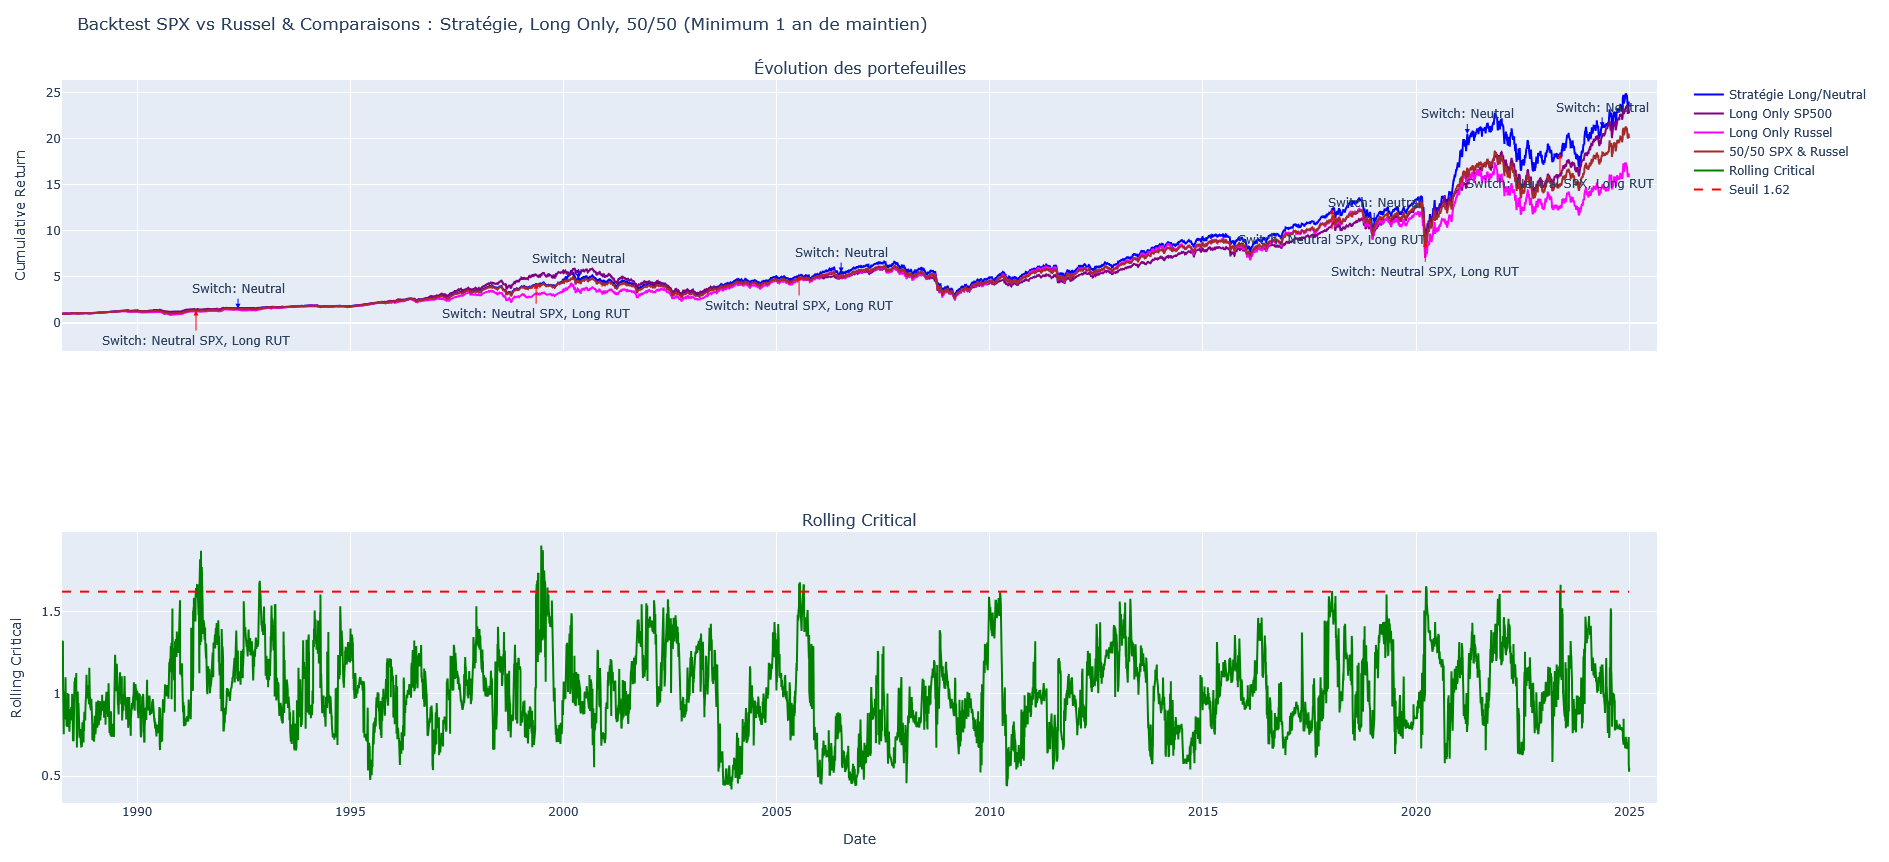
\includegraphics[width=0.8\textwidth]{img/backtest_long_neutral.png}
    \caption{Comparison of the performance of the over/under strategy (blue, purple, green) with the long only S\&P 500 portfolio (red),
        long only Russell 2000 portfolio (yellow), and 50/50 portfolio (black). The strategy is based on the Hurst
        exponent, where a value above 0.5 and positive momentum indicates an over exposition to the S\&P 500 (80\% of the
        portfolio) and under exposition to the Russell 2000 (20\% of the portfolio),
        a value above 0.5 and negative momentum indicates an under exposition to the S\&P 500 (20\% of the portfolio) and 
        over exposition to the Russell 2000 (80\% of the portfolio),
        and below 0.5 indicates a neutral position (50\% S\&P 500 and 50\% Russell 2000).
        The backtest period is from 1998-03-28 to 2025-02-28.}
    \label{fig:cumulative_performance}
\end{figure}

\FloatBarrier

\begin{table}[!h]
    \centering
    \pgfplotstabletypeset[
        columns={Strategy,Annualized Return,Annualized Volatility,Sharpe,Max Drawdown},
        columns/Strategy/.style={string type,column name=Strategy},
        columns/Annualized Return/.style={column name=Annualized Return},
        columns/Annualized Volatility/.style={column name=Annualized Volatility},
        columns/Sharpe/.style={column name=Sharpe},
        columns/Max Drawdown /.style={column name=Max Drawdown}
    ]{data/backtest_long_neutral_results.csv}
    \caption{Performance metrics of the over/under strategies (5 bps transaction fees) compared to the long only S\&P 500
    portfolio, long only Russell 2000 portfolio, 50/50 Russell /S\&P 500 portfolio.}
    \label{tab:performance_table}
\end{table}

We tested severals strategies to see how robust the results are, the ModifOverlap120 correspond to the estimation of a
Hurst based modified R/S statistic using a rolling window of 120 days, the TradOverlap120 correspond to the
traditional R/S statistic using a rolling window of 120 days, the ModifNonOverlap120 correspond to the estimation of a
Hurst based modified R/S statistic using a non overlapping rolling window of 120 days.
The results are shown in Table~\ref{tab:performance_table} and Figure~\ref{fig:cumulative_performance}.
All the strategies outperform the 50/50 portfolio and the long only Russell 2000 portfolio.
The ModifOverlap120 and TradOverlap120 strategy outperforms the long only S\&P 500 portfolio in terms of annualized return
but the long only S\&P 500 portfolio outperforms those strategies in terms of volatility, Sharpe and max drawdown.


\section{Conclusion}

In this paper, we examined the long-term memory and multifractal properties of major stock market indices using both
traditional and modified R/S analysis alongside Multifractal Detrended Fluctuation Analysis (MF-DFA). Our findings
suggest that, while most series display Hurst exponents greater than 0.5 implying some degree of persistence the
modified R/S approach indicates that only the Russell 2000 exhibits statistically significant long memory.
In contrast, the S\&P 500 shows a more subdued multifractal behavior, with a narrower spectrum and lower extremal Hölder
exponents. This difference may reflect underlying market microstructure characteristics, such as liquidity and the size
of constituent companies, but these interpretations should be treated with caution.

\section{Discussion}

It is important to emphasize that the methods used in our study both the static Hurst exponent and the multifractal
analysis are highly sensitive to the chosen data frequency, evaluation period, and potential structural breaks. The
apparent persistence observed in the Russell 2000, for instance, may be influenced by these factors, while the more
stable behavior seen in the S\&P 500 could result from its larger, more liquid market composition.

Furthermore, our analysis indicates that the multifractal parameters, such as the singularity spectrum, are subject to
sampling variability and estimation bias. The differences between the original and shuffled series, while suggestive of
distinct contributions from long-range correlations and heavy-tailed distributions, require further validation.

Additional tests, including robustness checks across different time frames and alternative multifractal estimation
methods, are necessary to substantiate our preliminary observations.

Overall, while our results provide an intriguing perspective on market dynamics and offer a foundation for a trading
strategy based on these multifractal measures, they should be interpreted with a degree of caution. Future research
should aim to extend this analysis to a broader set of assets (pair clustering) and refine the estimation techniques
to confirm the statistical significance of the observed multifractal effects.

\section{Appendix}

The critical values for the modified R/S test are provided in the table below. These values are used to assess whether the series exhibits long memory behavior based on the modified R/S statistic.

\begin{table}[ht!]
\centering
\begin{tabular}{|c|c|c|}
\hline
\textbf{Significance Level} & \textbf{critical value (modified R/S Statistic)} \\
\hline
0.005 & 2.098\\
0.05 & 1.747\\
0.10 & 1.620\\

\hline
\end{tabular}
\caption{critical values for the modified R/S Statistic (Lo, 1991)}
    \label{table:critical_values}
\end{table}

\begin{table}[h!]
    \centering
    \pgfplotstabletypeset[
        col sep=comma,
        header=true,
        string type,
        every head row/.style={before row=\hline, after row=\hline},
        every last row/.style={after row=\hline},
        columns/Ticker/.style={column name=Ticker, string type},
        columns/P-Value of prices/.style={column name=P-Value of Prices, fixed, precision=3},
        columns/P-Value of log differentiated return/.style={column name=P-Value of Log Differentiated Return, fixed, precision=3}
    ] {data/adf_results.csv}
    \caption{P-values from the Augmented Dickey-Fuller (ADF) test for stationarity. The P-value of prices refers to the Augmented Dickey Fuller test (ADF) on the original series,
     while the P-value of log-differentiated returns indicates the ADF test on log-differentiated returns. The null hypothesis is non-stationarity.}
    \label{tab:adf_results}
\end{table}

\FloatBarrier

\section{References}

Lo, A.W. (1991). \textit{\href{http://www.e-m-h.org/Lo\_\_91.pdf}{Long-Term Memory in Stock Market Prices}}. \\

Mignon, V. (2003). \textit{\href{https://www.persee.fr/doc/ecop_0249-4744_1998_num_132_1_5909}{Méthodes d'estimation de l'exposant de Hurst. Application aux rentabilités boursières}}, Économie \& Prévision.

Kantelhardt, J.W., Zschiegner, S.A., Koscielny-Bunde, E., Bunde, A., Havlin, S., \& Stanley, H.E. (2002). \textit{Multifractal Detrended Fluctuation Analysis of Nonstationary Time Series}. \textit{Physica A: Statistical Mechanics and its Applications}, 316(1--4), 87--114.

Andrews, D.W.K. (1991). \textit{\href{https://www.jstor.org/stable/2938229}{Heteroskedasticity and Autocorrelation Consistent Covariance Matrix Estimation}}. \textit{Econometrica}, 59(3), 817-858.

Mandelbrot, B.B. and Wallis, J.R. (1968). "Noah, Joseph, and Operational Hydrology", \textit{Water Resources Research}, vol. 4, pp. 909--918.

Mandelbrot, B.B. (1973). "Le problème de la réalité des cycles lents et le syndrome de Joseph", \textit{Economie Appliquée}, vol. 26, pp. 349--365.

Mandelbrot, B.B. and Wallis, J.R. (1969d). "Some Long-Run Properties of Geophysical Records", \textit{Water Resources Research}, vol. 5, pp. 321--340.

Mandelbrot, B.B. and Wallis, J.R. (1969e). "Robustness of the Rescaled Range R/S in the Measurement of Noncyclic Long-Run Statistical Dependence", \textit{Water Resources Research}, vol. 5, pp. 967--988.

Mandelbrot, B.B. and Taqqu, M.S. (1979). "Robust R/S Analysis of Long-Run Serial Correlation", \textit{Bulletin of the International Statistical Institute}, vol. 48, pp. 69--104.

\end{document}
